\documentclass[12pt, a4paper, UTF8]{article}
\usepackage{ctex}
\usepackage{indentfirst}
\usepackage{amsmath}
\usepackage{amsfonts}
\usepackage{amssymb}
\usepackage{graphicx}
\usepackage{geometry}
\usepackage{booktabs}
\usepackage{caption}
\usepackage{subcaption}
\usepackage{hyperref}
\usepackage{siunitx}
\usepackage{enumitem}
\usepackage{xeCJK}
\usepackage{array}
\usepackage{listings}
\usepackage{xcolor}
\usepackage{epstopdf}
\usepackage{float}

\hypersetup{hidelinks}

\title{实验报告：\\7nm FinFET 器件电性校准（Part II）}
\author{作者：徐子翔 \hspace{0.2cm} 郦查德}
\date{\today}

\begin{document}

\maketitle

\section{实验目的}
本实验旨在在几何结构已校准的基础上，结合参考数据对 7nm FinFET 的电性模型进行校准，确保 TCAD 的 C--V、I--V 曲线与 SPICE 数据一致，获得可信的器件电学参数，为后续器件设计与性能评估提供基础。


\section{长沟 CV 校准}
\subsection{实验原理}
为降低寄生电容干扰，采用两种沟长的 CV 数据作差，提取“纯净沟道电容”。对同一器件、不同沟长 $L$，可写出
\begin{equation}
C_{gc}(L, V_g)=C_{ch}(V_g)\cdot L + C_{par}(V_g)
\end{equation}
其中 $C_{gc}=C_{gg}-C_{gb}=C_{gs}+C_{gd}$。由两条曲线斜率得到单位沟道长度电容
\begin{equation}
C_{ch}(V_g)=\frac{C_{gc}(L_2,V_g)-C_{gc}(L_1,V_g)}{L_2-L_1}
\end{equation}
此外，量子限域效应会显著影响电容，需要在仿真中启用 DG（Density Gradient）模型进行校准。

\subsection{操作步骤}
\begin{enumerate}
    \item 在本地目录建立长沟工程，生成两种长沟器件（如 $L_{design}=20/36\,\si{nm}$）结构与 CV 仿真模块，并输出 $C_{gg}$ 曲线,采用工具处理数据。
    \item 优先对齐强反型区电容，调节参数oxideThickness，highKThickness。
    \item 再对齐耗尽区电容，调节参数channelDoping，wellDoping。
    \item 功函数用于平移 C--V 曲线，用测量软件测出水平偏差，修改 $E_w$。
\end{enumerate}

\begin{table}[H]
    \centering
    \large
    \begin{tabular}{lcc} % l: 左对齐, c: 居中对齐
        \toprule
        \textbf{参数名} & \textbf{最终值} \\
        \midrule
        oxideThickness & 0.900 nm \\
        highKThickness & 1.30 nm \\
        channelDoping & 1.000E14 $cm^{-3}$ \\
        wellDoping & 1.000E17 $cm^{-3}$\\
        $E_w$ & -0.3 ev \\
        \bottomrule
    \end{tabular}
\end{table}

长沟 CV 校准前后对比如图~\ref{fig:longcv-compare}所示。
\begin{figure}[H]
    \centering
    \begin{subfigure}[t]{0.48\textwidth}
        \centering
        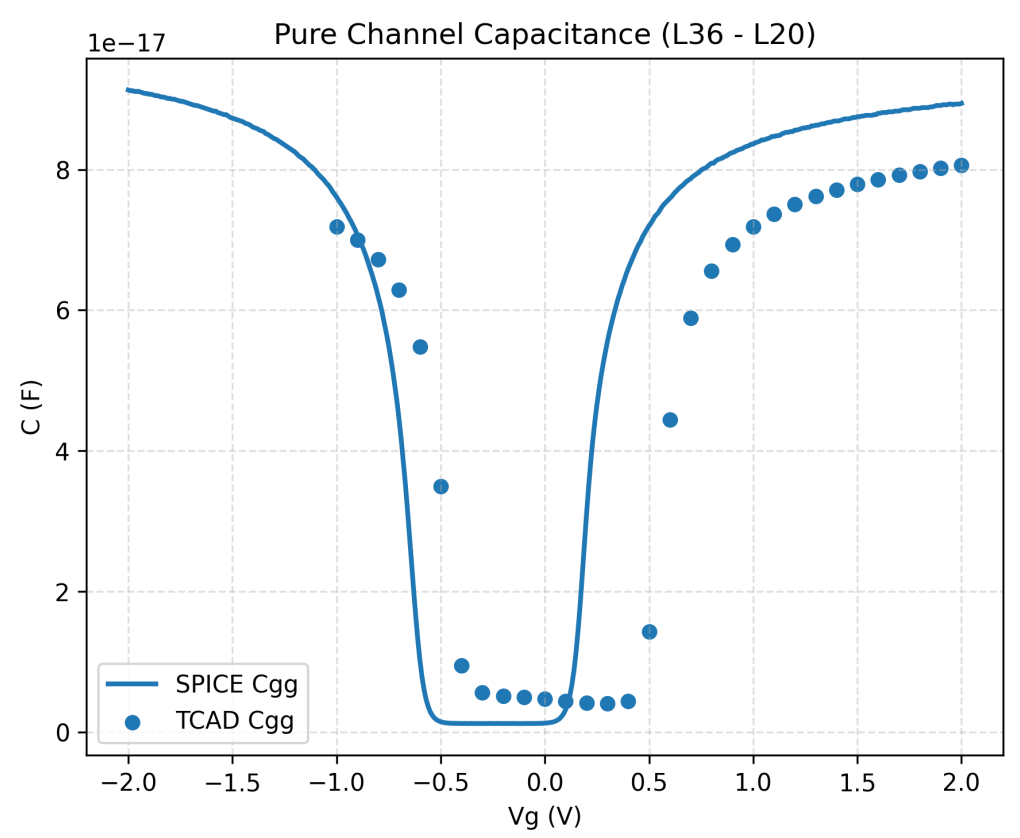
\includegraphics[width=\textwidth]{image/LongChannelCV_Initial.png}
        \caption{未校准}
        \label{fig:longcv-initial}
    \end{subfigure}
    \hfill
    \begin{subfigure}[t]{0.48\textwidth}
        \centering
        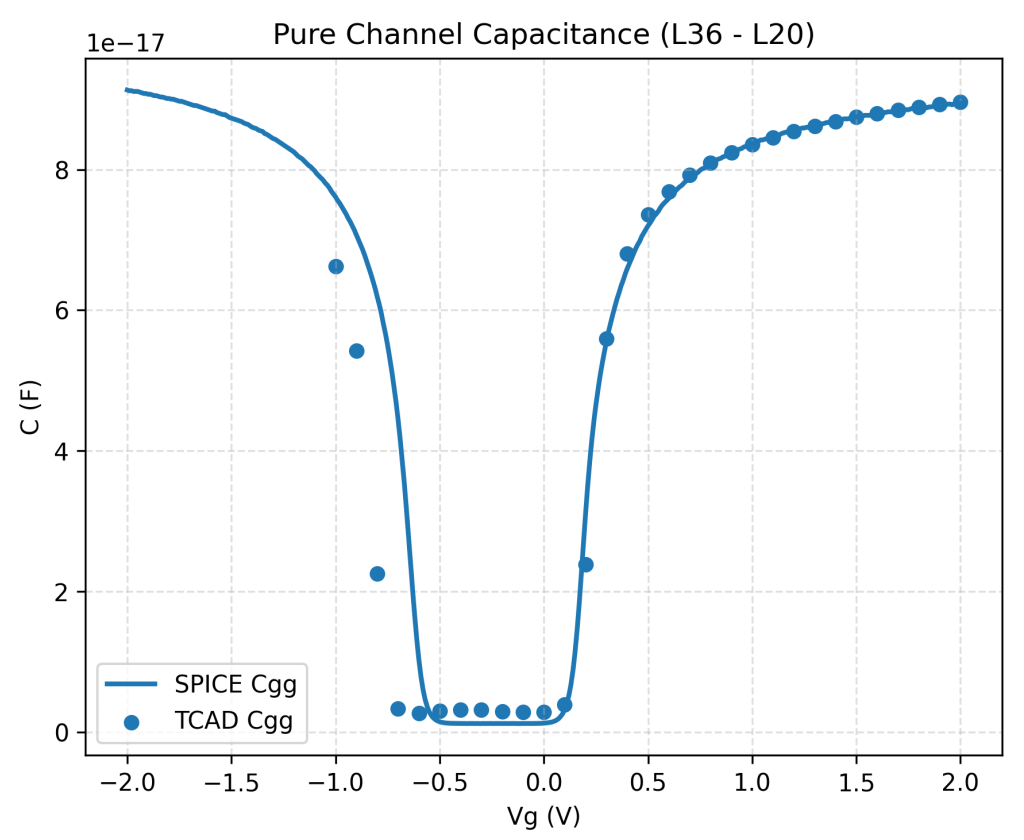
\includegraphics[width=\textwidth]{image/LongChannelCV_Final.png}
        \caption{校准后}
        \label{fig:longcv-final}
    \end{subfigure}
    \caption{长沟器件 $C_{gg}$--$V_g$ 曲线校准前后对比}
    \label{fig:longcv-compare}
\end{figure}

\section{长沟低场迁移率校准}
\subsection{实验原理}
本节目标是提取并校准器件本征的低场（横向电场）迁移率。为排除源漏接触、外延、沟道延伸区等寄生区域的影响，采用 Split CV（多沟长拆分）方法：先得到“纯净沟道”的反型电荷 $Q_{inv}$，再从多沟长的电阻拆分得到沟道有效迁移率 $\mu_{ch,eff}$。

\noindent\textbf{(1) Split Step 1：端口拆分}
\begin{equation}
C_{gg}=C_{gc}+C_{gb}
\end{equation}
其中沟道相关的栅电容为
\begin{equation}
C_{gc}=C_{gg}-C_{gb}=C_{gs}+C_{gd}
\end{equation}

\noindent\textbf{(2) Split Step 2：提取单位沟道长度电容与电荷}
对同一类 FinFET，仅改变沟道长度 $L$，可近似认为 $C_{gc}$ 与 $L$ 呈一阶线性关系：
\begin{equation}
C_{gc}(L,V_g)=C_{ch}(V_g)\cdot L + C_{ext}(V_g)
\end{equation}
其中 $C_{ch}(V_g)$ 为单位沟道长度的“纯净沟道电容”（由斜率得到）：
\begin{equation}
C_{ch}(V_g)=\frac{\partial C_{gc}(L,V_g)}{\partial L}\approx \frac{C_{gc}(L_2,V_g)-C_{gc}(L_1,V_g)}{L_2-L_1}
\end{equation}
由 $C_{ch}$ 积分得到单位沟道长度的反型层电荷：
\begin{equation}
Q_{inv}(V_g)=\int_{V_{g0}}^{V_g} C_{ch}(V)\,dV
\end{equation}
其中 $V_{g0}$ 可选取在弱反型起始或参考电压点。

\noindent\textbf{(3) Split Step 3：提取低场迁移率}
\\理想状态下，在小漏压 $V_{ds}$ 的线性区，可由漂移电流关系写出
\begin{equation}
I_{ds}(V_g)=\mu_{ch,eff}(V_g)\,\frac{Q_{inv}(V_g)}{L}\,V_{ds}
\end{equation}
因此沟道电阻为
\begin{equation}
R_{ch}(L,V_g)=\frac{L}{\mu_{ch,eff}(V_g)\,Q_{inv}(V_g)}
\end{equation}
考虑源漏串联电阻（寄生电阻）$R_{sd}$，总电阻模型为
\begin{equation}
R_{tot}(L,V_g)=\frac{V_{ds}}{I_{ds}}=R_{ch}(L,V_g)+R_{sd}(V_g)=\frac{L}{\mu_{ch,eff}(V_g)\,Q_{inv}(V_g)}+R_{sd}(V_g)
\end{equation}
对不同沟长 $L$ 的 $R_{tot}$ 做线性拟合，得到单位沟道长度电阻（斜率）：
\begin{equation}
\frac{\partial R_{tot}(L,V_g)}{\partial L}=\frac{1}{\mu_{ch,eff}(V_g)\,Q_{inv}(V_g)}
\end{equation}
实际计算时常用差分近似斜率：
\begin{equation}
\frac{\partial R_{tot}(L,V_g)}{\partial L}\approx \frac{R_{tot}(L_2,V_g)-R_{tot}(L_1,V_g)}{L_2-L_1}
\end{equation}
从而低场（有效）迁移率可由
\begin{equation}
\mu_{ch,eff}(V_g)=\frac{1}{Q_{inv}(V_g)}\left(\frac{\partial R_{tot}(L,V_g)}{\partial L}\right)^{-1}
\end{equation}
得到。最后通过消去 $V_g$（用 $Q_{inv}$ 或工具换算得到的 $N_{inv}$ 作为横轴），即可得到本征低场迁移率 $\mu_{ch,eff}(Q_{inv})$ 的校准曲线。

\noindent\textbf{(4) Matthiessen 低场迁移率模型}
在漂移扩散框架下，低场迁移率常按 Matthiessen 规则由多种散射/退化机制并联叠加：
\begin{equation}
\frac{1}{\mu_{LF}}=\frac{1}{\mu^{\mathrm{bulk}}}+\frac{1}{\mu^{\mathrm{surf}}}+\frac{1}{\mu^{\mathrm{deg}}}
\end{equation}
其中体迁移率 $\mu^{\mathrm{bulk}}$ 由晶格（声子）散射与库仑（杂质）散射共同决定：
\begin{equation}
\frac{1}{\mu^{\mathrm{bulk}}}=\frac{1}{\mu^{L}}+\frac{1}{\mu^{\mathrm{IM}}}
\end{equation}
其中库仑散射迁移率 $\mu^{\mathrm{IM}}$ 可在 ``bulk'' 与 ``surface'' 两种模型间切换：
\begin{equation}
\mu^{\mathrm{IM}}=
\begin{cases}
\mu^{\mathrm{IM,bulk}}, & \texttt{enableSurfaceImpurity}=\texttt{false}\\
\mu^{\mathrm{IM,surf}}, & \texttt{enableSurfaceImpurity}=\texttt{true}
\end{cases}
\end{equation}

当启用表面库仑散射（Mujtaba 模型）时：
\begin{equation}
\mu^{\mathrm{IM,surf}}=\left(1-\exp\left(-\frac{d}{d_0}\right)\right)\mu^{\mathrm{IM,bulk}}+\exp\left(-\frac{d}{d_0}\right)\left(f\mu^{\mathrm{IM,bulk}}+(1-f)\mu^{\mathrm{IM2D}}\right)
\end{equation}
\begin{equation}
f=\left(1+\exp\left(S_F\frac{\mathcal{F}^{2/3}}{T/(300\,\mathrm{K})}+S_t\frac{1}{(t_B/t_0)^2\,T/(300\,\mathrm{K})}-\lambda\right)\right)^{-1}
\end{equation}

其中二维库仑散射迁移率 $\mu^{\mathrm{IM2D}}$写为：
\begin{equation}
\frac{1}{\mu^{\mathrm{IM2D}}}=\operatorname{erf}\left(\frac{t_B}{t_1}\right)\left(\frac{1}{\mu^{\mathrm{acc}}}+\frac{1}{\mu^{\mathrm{inv}}}\right)
\end{equation}
\begin{equation}
\mu^{\mathrm{acc}}=\sqrt{\left(\mu_{1}^{\mathrm{acc}}\right)^2+\left(\mu_{2}^{\mathrm{acc}}\right)^2G},\qquad
\mu^{\mathrm{inv}}=\sqrt{\left(\mu_{1}^{\mathrm{inv}}\right)^2+\left(\mu_{2}^{\mathrm{inv}}\right)^2}
\end{equation}
并给出部分迁移率表达式：
\begin{align}
\mu_{1}^{\mathrm{acc}}&=\mu_{10}^{\mathrm{acc}}\left(\frac{T}{300\,\mathrm{K}}\right)^{\alpha_{\mathrm{acc}1}}\left(\frac{N_{\mathrm{Dref}}}{N_{\mathrm{acc}}}\right)^{\beta_{\mathrm{acc}1}}\left(\frac{\nu}{N_{\mathrm{ref}}}\right)^{\gamma_{\mathrm{acc}}}\\
\mu_{2}^{\mathrm{acc}}&=\mu_{20}^{\mathrm{acc}}\left(\frac{T}{300\,\mathrm{K}}\right)^{\alpha_{\mathrm{acc}2}}\left(\frac{N_{\mathrm{Dref}}}{N_{\mathrm{acc}}}\right)^{\beta_{\mathrm{acc}2}}\\
\mu_{1}^{\mathrm{inv}}&=\mu_{10}^{\mathrm{inv}}\left(\frac{T}{300\,\mathrm{K}}\right)^{\alpha_{\mathrm{inv}1}}\left(\frac{N_{\mathrm{Dref}}}{N_{\mathrm{inv}}}\right)^{\beta_{\mathrm{inv}1}}\left(\frac{\nu}{N_{\mathrm{ref}}}\right)^{\gamma_{\mathrm{inv}}}\\
\mu_{2}^{\mathrm{inv}}&=\mu_{20}^{\mathrm{inv}}\left(\frac{T}{300\,\mathrm{K}}\right)^{\alpha_{\mathrm{inv}2}}\left(\frac{N_{\mathrm{Dref}}}{N_{\mathrm{inv}}}\right)^{\beta_{\mathrm{inv}2}}
\end{align}

表面散射迁移率由 Lombardi 模型与 Reggiani 模型共同决定：
\begin{equation}
\frac{1}{\mu^{\mathrm{surf}}}=\frac{1}{\mu^{\mathrm{surf},L}}+\frac{1}{\mu^{\mathrm{surf},R}}
\end{equation}

\noindent\textbf{(5) Lombardi 表面迁移率模型}
Lombardi 模型将表面声子散射与表面粗糙散射按 Matthiessen 规则组合。对 Lombardi 表面散射项可写为
\begin{equation}
\frac{1}{\mu^{\mathrm{surf},L}}=
\left(\frac{(1-\Phi^{AC})\exp\left(-\frac{d}{d_0}\right)}{\mu_1^{ac}}+\frac{1}{\mu_2^{ac}}\right)
+\frac{(1-\Phi^{SR})\exp\left(-\frac{d}{d_0}\right)}{\mu^{sr}}
\end{equation}
模型中的 $\mu_1^{ac}$ 与 $\mu^{sr}$ 采用如下形式：
\begin{equation}
\mu_1^{ac}=\frac{B}{\mathcal{F}}+\frac{C\cdot\left(\alpha_A\mathcal{N}_A^{\beta_A}+\alpha_D\mathcal{N}_D^{\beta_D}\right)^{L}}{\mathcal{F}^{1/3}\cdot\left(\frac{T_L}{300\,\mathrm{K}}\right)^{\eta}}
\end{equation}
\begin{equation}
\mu^{sr}=\frac{\left(\gamma_A\mathcal{N}_A^{\delta_A}+\gamma_D\mathcal{N}_D^{\delta_D}\right)^{L_{sr}}}{\frac{\mathcal{F}^{\alpha}}{D}+\frac{\mathcal{F}^{3}}{E}}
\end{equation}
并定义归一化掺杂变量
\begin{equation}
\mathcal{N}_A=\frac{N_A}{N_0},\qquad \mathcal{N}_D=\frac{N_D}{N_0}
\end{equation}
其中 $\mathcal{F}$ 为有效场相关量，$T_L$ 为晶格温度，其余参数为模型拟合系数。

\subsection{操作步骤}
\begin{enumerate}
    \item 在长沟工程中建立两种沟长器件的线性区 I--V 仿真后使用工具提取出迁移率曲线。
    \item 仅关注强反型区的迁移率曲线，并结合 Matthiessen 规则与表面散射模型参数进行对齐。
\end{enumerate}

\begin{table}[H]
    \centering
    \large
    \begin{tabular}{lcc} % l: 左对齐, c: 居中对齐
        \toprule
        \textbf{参数名} & \textbf{初始值} & \textbf{最终值} \\
        \midrule
        uinv10 & 135 cm²/V·s & 270 cm²/V·s \\
        uinv20 & 40 cm²/V·s & 80 cm²/V·s \\
        uAC2uref & 250 cm²/V·s & 400 cm²/V·s \\
        B300 & 4.75 e7 cm²/V·s & 4.5 e9 cm²/V·s\\
        C300 &580 cm²/V·s & 1000 cm²/V·s\\
        D300 & 5 e13 cm²/V·s & 3.4 e14 cm²/V·s\\
        \bottomrule
    \end{tabular}
\end{table}


长沟低场迁移率校准前后对比如图~\ref{fig:longmiu-compare}所示。
\begin{figure}[H]
    \centering
    \begin{subfigure}[t]{0.48\textwidth}
        \centering
        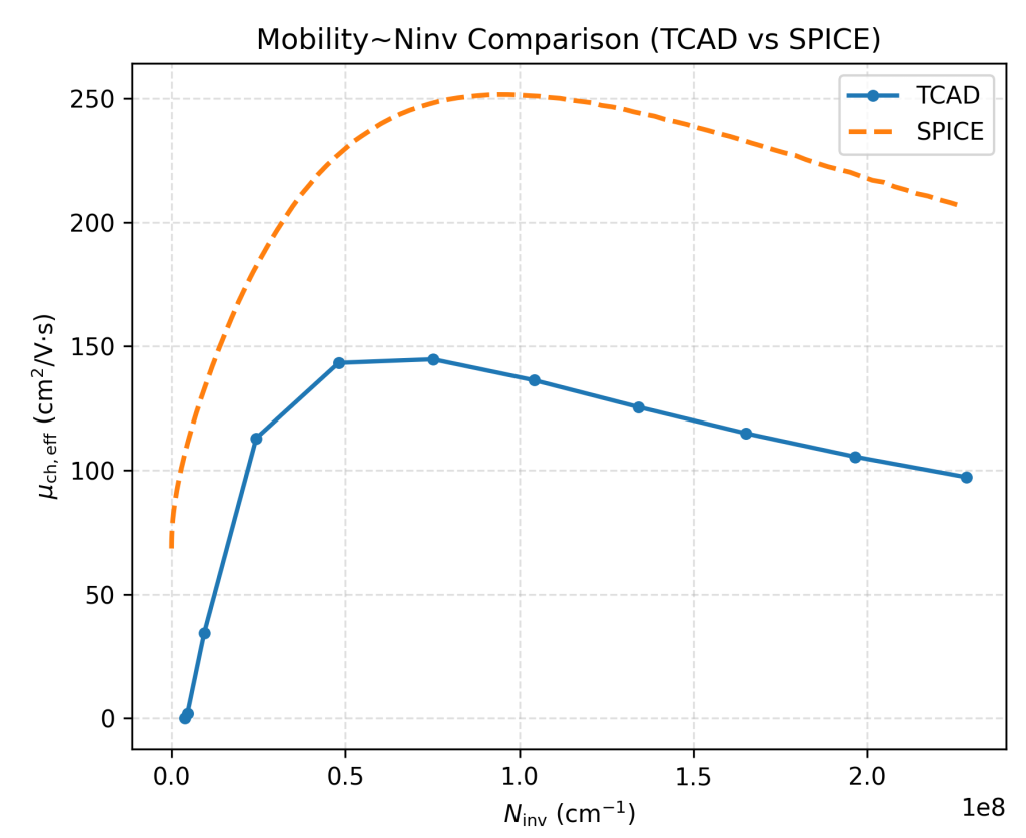
\includegraphics[width=\textwidth]{image/LongChannelMiu_Initial.png}
        \caption{未校准}
        \label{fig:longmiu-initial}
    \end{subfigure}
    \hfill
    \begin{subfigure}[t]{0.48\textwidth}
        \centering
        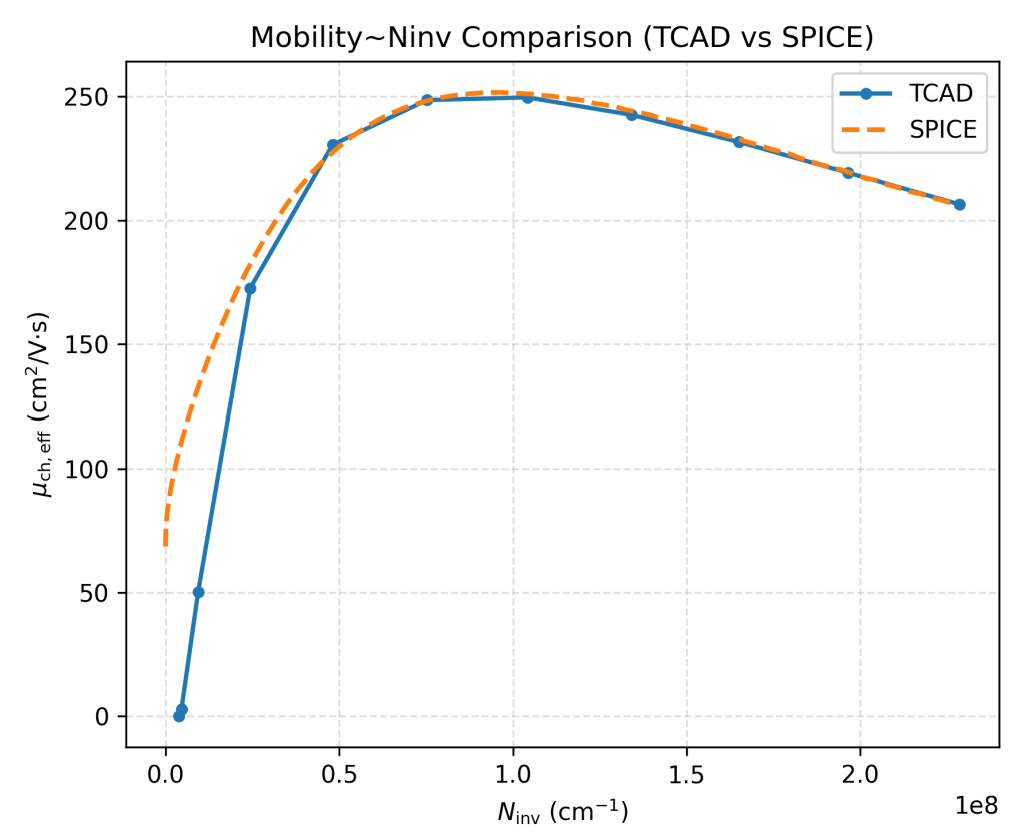
\includegraphics[width=\textwidth]{image/LongChannelMiu_Final.png}
        \caption{校准后}
        \label{fig:longmiu-final}
    \end{subfigure}
    \caption{长沟低场迁移率提取与校准前后对比}
    \label{fig:longmiu-compare}
\end{figure}

\section{短沟 CV 校准}

\subsection{实验原理}
\subsection{操作步骤}


\section{短沟 IV 校准}

\subsection{实验原理}
\subsection{操作步骤}

\section{思考题}
\subsection{为什么不能直接用一条长沟器件的IV曲线提取长沟迁移率？}
答：直接使用单条长沟器件的 IV 曲线提取迁移率会受到寄生电阻（如源漏接触电阻、外延区电阻等）的影响，导致提取的迁移率不准确。通过两条不同长度沟道做差方法，消除寄生电阻的影响，从而得到更准确的迁移率。
\subsection{为何不关注除强反型区以外的其它区的迁移率和Qinv？}
答：强反型区载流子移动以漂移为主，迁移率对器件性能影响最大；而弱反型区和积累区载流子移动以扩散为主，迁移率对器件性能影响小。而Qinv由两个不同长度沟道器件做差得到，$C_gc$-$V_g$图中其他区域两条曲线几乎重叠，校准意义不大。

\subsection{请阅读Minimos手册中弹道输运模型相关内容，结合弹道输运机制，思考参数p对于不同
沟长器件的取值大小关系}
答：

\subsection{阅读手册，尝试在实验报告中分析CV仿真中Cgg和Cgd的计算原理}
答：
在 GTS Minimos-NT 等 TCAD 仿真工具中，器件的电容并非通过简单的准静态电荷求导 ($C = dQ/dV$) 获得，而是通过\textbf{AC 小信号分析}从多端口导纳矩阵（Admittance Matrix, Y矩阵）中提取的。这种方法能够更准确地捕捉非准静态效应和频率相关特性。

对于一个 MOSFET 器件，通常被视为一个四端口网络（Gate, Drain, Source, Bulk）。在给定的 DC 工作点（Bias Point）上，向端口 $j$ 施加一个微小的正弦电压扰动 $\tilde{v}_j = \Delta V_j e^{j\omega t}$，在端口 $i$ 测量引起的小信号电流 $\tilde{i}_i$。

\textbf{(a) Y 矩阵与导纳定义}

多端口系统的电流-电压关系可以表示为：
\begin{equation}
\begin{bmatrix}
\tilde{i}_g \\
\tilde{i}_d \\
\tilde{i}_s \\
\tilde{i}_b
\end{bmatrix}
=
\begin{bmatrix}
Y_{gg} & Y_{gd} & Y_{gs} & Y_{gb} \\
Y_{dg} & Y_{dd} & Y_{ds} & Y_{db} \\
Y_{sg} & Y_{sd} & Y_{ss} & Y_{sb} \\
Y_{bg} & Y_{bd} & Y_{bs} & Y_{bb}
\end{bmatrix}
\begin{bmatrix}
\tilde{v}_g \\
\tilde{v}_d \\
\tilde{v}_s \\
\tilde{v}_b
\end{bmatrix}
\end{equation}

其中每一个复导纳元素 $Y_{ij}$ 都可以分解为实部（电导 $G$）和虚部（电感或电容）：
\begin{equation}
Y_{ij} = G_{ij} + j\omega C_{ij}
\end{equation}
这里 $\omega = 2\pi f$ 是交流信号的角频率。

\textbf{(b) $C_{gg}$ 与 $C_{gd}$ 的提取原理}

通过上述矩阵关系，我们可以精确定义电容分量：
\begin{enumerate}
\item \textbf{总栅极电容 $C_{gg}$ (Gate Self-Capacitance)}
$C_{gg}$ 定义为当栅极电压变化时，栅极端口流入的总电荷变化率。它对应于 Y 矩阵中栅极端口的自导纳（Self-admittance）的虚部：
\begin{equation}
C_{gg} = \frac{\text{Im}(Y_{gg})}{\omega}
\end{equation}
在物理上，$C_{gg}$ 是所有跨导电容之和：$C_{gg} = C_{gs} + C_{gd} + C_{gb}$。它反映了栅极对整个器件沟道电荷的控制能力。

\item \textbf{栅漏反向传输电容 $C_{gd}$ (Gate-Drain Trans-capacitance)}
$C_{gd}$ 反映了漏端电压变化在栅极引起的感应电荷变化。根据 Y 矩阵定义：
\begin{equation}
\tilde{i}_g = Y_{gg}\tilde{v}_g + Y_{gd}\tilde{v}_d + \dots
\end{equation}
当固定其他电极电压（$\tilde{v}_g=0, \tilde{v}_s=0, \tilde{v}_b=0$），仅在漏端施加扰动时：
\begin{equation}
C_{gd} = - \frac{\text{Im}(Y_{gd})}{\omega}
\end{equation}
\textbf{注意：} 互电容（Trans-capacitance）前通常带有负号，这是因为流入端口 $i$ 的电流是由另一端口电压升高导致的电荷重新分配引起的。

\end{enumerate}

\textbf{(c) 仿真计算流程简述}

在 Minimos-NT 中，计算步骤如下：
\begin{enumerate}
    \item \textbf{DC 求解}：获得稳定的电势 $\psi$ 和载流子浓度 $n, p$ 分布。
    \item \textbf{线性化求解}：对半导体基本方程（泊松方程、连续性方程）进行 Fréchet 微分，建立小信号系统矩阵。
    \item \textbf{AC 扰动}：在指定频率下求解线性方程组，直接得到各端口电流响应。
    \item \textbf{参数提取}：通过 $C_{ij} = \text{Im}(Y_{ij})/\omega$ 输出电容值。
\end{enumerate}

\subsection{Split CV时若采用短沟的器件，会对迁移率校准有什么影响？}
答：
在本实验流程中若采用短沟的器件，\textbf{“低场漂移/局域迁移率”假设会开始失效}：由于 $L$ 很小，即使选取较小 $V_{ds}$，沟道横向电场仍可能很大（$E\sim V_{ds}/L$），载流子更容易进入速度饱和或准弹道（非定域）输运区，电流不再严格满足长沟线性区的
\begin{equation}
I_d\propto \mu\,\frac{Q_{inv}}{L}\,V_{ds}
\end{equation}
从而用短沟器件按 Split CV 形式反推得到的 $\mu_{ch,eff}$ 往往变成\textbf{把速度饱和、弹道限制等效应“混进去”的等效迁移率}：它会随 $V_{gs}$、$V_{ds}$ 呈现更强的偏置依赖。若直接用该曲线去校准低场迁移率模型参数，会把短沟输运效应误吸收到 $\mu$ 参数中，反而破坏长沟与短沟的一致性。

因此更合理的策略是：\textbf{低场迁移率参数仍以长沟器件为主校准}；短沟器件的偏差主要通过\textbf{高场迁移率/速度饱和}与\textbf{弹道输运模型（如参数 $p$）}等短沟相关机制，在短沟 IV迭代中完成对齐。

\subsection{如果不给定校准好的DG模型参数，将DG模型的校准考虑到整个TCAD校准流程中，请问如何重新设计整个校准的流程？}

\subsection{校准短沟低场迁移率和串联电阻时，采用恒定电流法计算Vt，会怎么样？}

\end{document}
